%
%   Copyright 2013 Katarzyna Szawan <kat.szwn@gmail.com>
%       and Michał Rus <m@michalrus.com>
%
%   Licensed under the Apache License, Version 2.0 (the "License");
%   you may not use this file except in compliance with the License.
%   You may obtain a copy of the License at
%
%       http://www.apache.org/licenses/LICENSE-2.0
%
%   Unless required by applicable law or agreed to in writing, software
%   distributed under the License is distributed on an "AS IS" BASIS,
%   WITHOUT WARRANTIES OR CONDITIONS OF ANY KIND, either express or implied.
%   See the License for the specific language governing permissions and
%   limitations under the License.
%

\begin{frame}
\frametitle{System do tworzenia map myśli}

\begin{columns}[c]
	\begin{column}[t]{.45\textwidth}
		\vskip-7.5em
		\begin{enumerate}
			\item Działanie w systemie Android.
			\only<2->{\item Kompatybilność z programem XMind --- eksport i import.}
			\only<3->{\item Tworzenie map, edycja zawartości węzłów, usuwanie węzłów i ich dzieci.}
			\only<4->{\item Kolaboracja online.}
			\only<5->{\item Synchronizacja offline.}
			
		\end{enumerate}
	\end{column}
	\begin{column}{.45\textwidth}
		\begin{figure}
			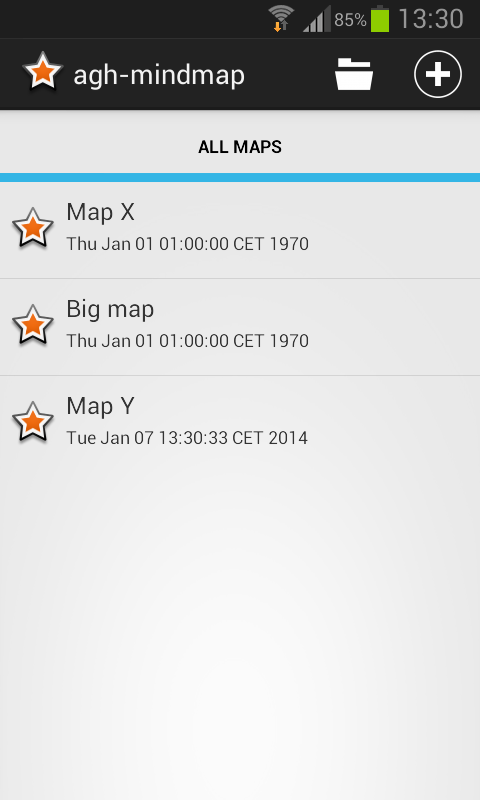
\includegraphics[height=6cm]{graphics-screenshot-list}
		\end{figure}
	\end{column}
\end{columns}

\end{frame}
